%************************************************
\chapter{Assessment of current Business Process Management Solutions}\label{ch:assessment}
%************************************************

The lack of flexibility in handling event subscription in business processes has been outlined in the previous chapters and a set of extended requirements to process management solutions have been presented.
In this section I take a closer look at the capabilities of current solutions with regards to the event occurrence scenarios to get a better understanding of the issues that arise when working with event subscription in business processes.
The assessment will be carried out using BPMN and Camunda, a state-of-the art and widely adopted business process engine.
The main goal is to identify and illustrate the shortcomings of the current process technology stack. These shortcomings will be referenced in addition to the presented requirements to develop a more refined subscription handling model in the following chapter. \todo[inline]{"subscription handling model"?}

\todo[inline]{which functionality should be evaluated exactly?: all occurrence scenarios, but no buffer policies. The buffer will always store the last version of the event and also deliver that version.}

\section{BPMN Models in presence of the Event Occurrence Scenarios}
Chapter X has revealed that processes can run into deadlocks if events do not occur at the right time \todo[inline]{.}
\begin{figure}[]
	\myfloatalign
	{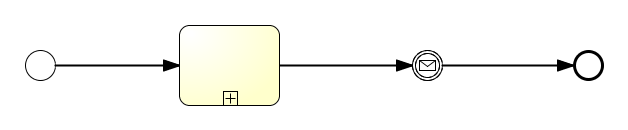
\includegraphics[width=1\linewidth]{chapters/assessment/process-with-intermediate-event.png}}
	\caption{Abstract Process using an Intermediate Catch Event}\label{fig:abstract-process-with-event}
\end{figure}

\autoref{fig:abstract-process-with-event} shows a generalized process that uses an Intermediate Catch Event just before process termination.
In this section I first describe for each Event Occurrence Scenario how this simple event implementation behaves in presence of the given scenario. I then evaluate if it is feasible to create a BPMN model that is free from deadlock in these situations. 

\paragraph{Scenario O1: The event occurs after the enabling of the BPMN event}
\begin{figure}[]
	\myfloatalign
	{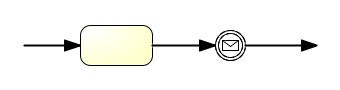
\includegraphics[width=1\linewidth]{chapters/assessment/standard-intermediate-event.png}}
	\caption{Standard Intermediate Catch Event}\label{fig:excerpt-standard-event}
\end{figure}

The first scenario represents the most simple case, that is also natively supported by the BPMN 2.0 specification. When the event occurs after the Event element has been enabled, the event will be received and the process can proceed normally. The use of a standard Intermediate Catch Event does suffice to cover this situation.

\paragraph{Scenario O2: The event does not occur}
\begin{figure}[]
	\myfloatalign
	{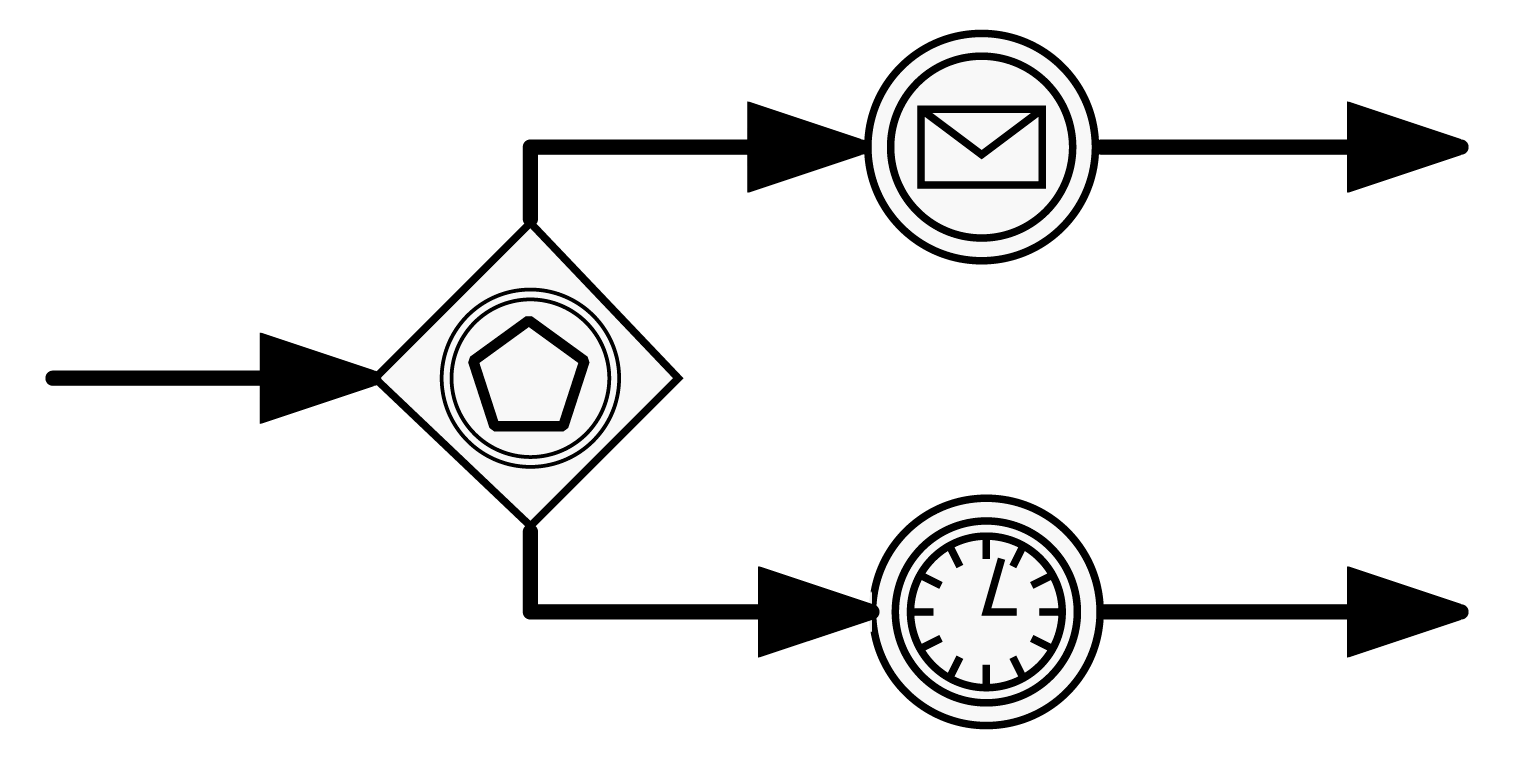
\includegraphics[width=1\linewidth]{chapters/assessment/parallel-timer-event.png}}
	\caption{Intermediate Event with a parallel Timer Event}\label{fig:excerpt-event-with-timer}
\end{figure}
\todo[inline]{alternatively: a receive task with boundary timer event}

In certain situations an event might not occur at all. Given a basic event implementation like in \autoref{fig:abstract-process-with-event}, the process flow will get to a halt once it reaches the Intermediate Catch Event and will not be able to proceed. While, depending on the process design, this might be the desired behavior, in many situations this is not acceptable.

Let's consider a process that is supposed to wait for approval for a certain amount of time and trigger an additional request if the approval has not been issued before the deadline. \autoref{fig:excerpt-event-with-timer} shows how this behavior can be implemented using an Event-based Gateway which puts a Timer Event in parallel to the Intermediate Catch Event. This extension will make sure that a process does not run into a deadlock state if the expected event does not occur.

\todo[inline]{I mention an example, but that example is not exactly illustrated in the process}
\todo[inline]{according to the spec: what exactly will happen to the active catch event once the timer fires?}


\paragraph{Scenario O3: Occurrence between Process instantiation and the enabling of the BPMN event}
\begin{figure}[]
	\myfloatalign
	{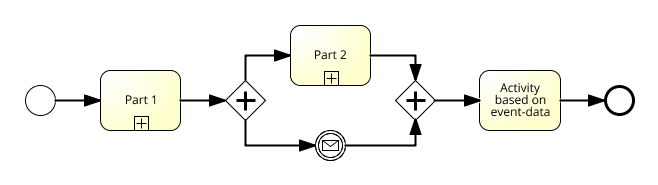
\includegraphics[width=1\linewidth]{chapters/assessment/parallel-gateway-early-subscription.png}}
	\caption{Event Element in parallel process flow}\label{fig:excerpt-parallel-gateway-event}
\end{figure}

In case the event occurs during process execution, but before the BPMN event element is enabled and thus listening for events, the occurrence will not be considered in the execution. The process will get stuck at the Event Process Element as if the event did not happen at all.
To avoid a deadlock in this scenario, a solution is to execute the Intermediate Catch Event in parallel to the rest of the process flow using a Parallel Gateway. This is illustrated in \autoref{fig:excerpt-parallel-gateway-event}. The time of subscription to the event can be controlled by the position of the parallel split: To implement an event subscription right after process instantiation, the Parallel Gateway has to be the first element after the Start Event (that means \textit{Part~1} in the illustration is empty). To implement event subscription at a specific point during process execution, part of the process can execute before reaching the Parallel Gateway. In \autoref{fig:excerpt-parallel-gateway-event}, the event may occur at any time during the execution of the collapsed sub-process \textit{Part~2}. 

\paragraph{Scenarios O4 and O5: Before Process Instantiation}
\begin{figure}[]
	\myfloatalign
	{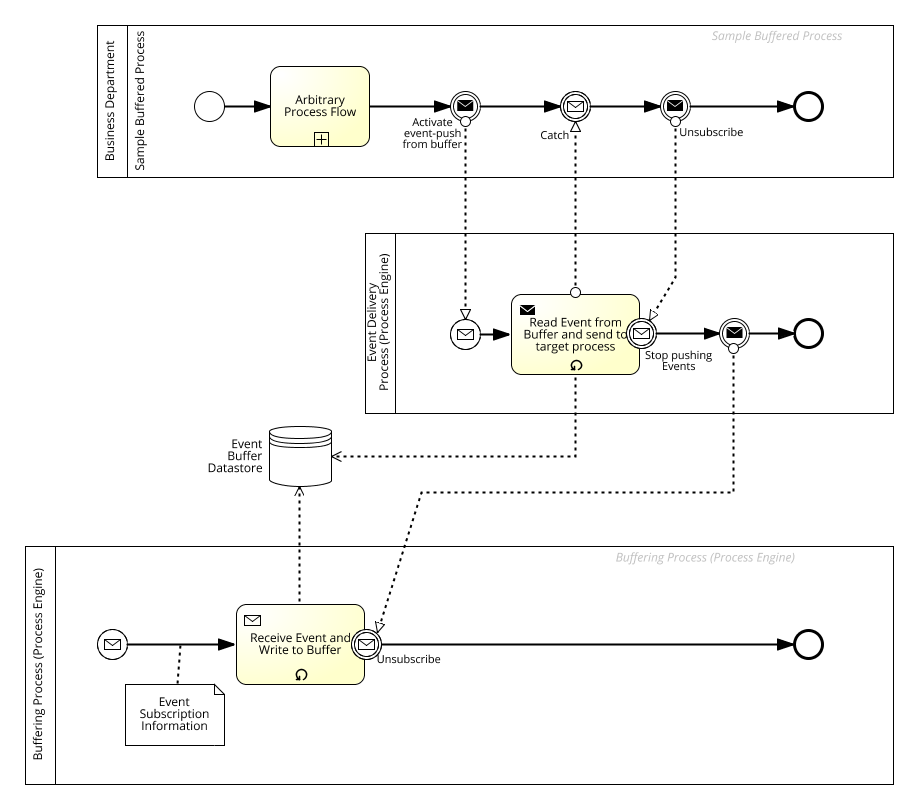
\includegraphics[width=1\linewidth]{chapters/assessment/aux-buffer-process.png}}
	\caption{Event Buffering through an auxiliary Buffering Process}\label{fig:aux-buffering-process}
\end{figure}

Any Events that happen before process instantiation will not be considered in a standard Intermediate Catch Event. That applies to both scenarios, the occurrence between deployment and instantiation (\textit{O4}) and an occurrence time before the deployment of the process in the Process Engine (\textit{O5}).

To create a Process Model that allows to catch an event before the process instance exists, three new elements are introduced: (1) An additional \textit{Auxiliary Buffering Process} that can catch an incoming event, (2) an \textit{Event~Buffer}, a temporary data-store that keeps event data until required by the \textit{Original~Process}, (3) an \textit{Auxiliary Event Delivery Process}, that retrieves events from the buffer and makes them available to the \textit{Original~Process}.
\autoref{fig:aux-buffering-process} reveals the interaction of the \textit{Original Process}, the two auxiliary processes and the data-store. To start listening for an event, the \textit{Auxiliary Buffering Process} has to be instantiated through the a message start event containing the information necessary for the event subscription. The process starts listening for the event and writes the received event to the temporary data-store. 
The given process design is able to handle multiple event occurrences, because the receiving activity is looping. The buffering process terminates once the \textit{Unsubscribe} event is received.

\todo[inline]{how should the ABP be started? manually?}

The \textit{Original Process} can be started any time after the buffering process. In \autoref{fig:aux-buffering-process}, the Intermediate Catch Event has been explicitly split into three events: An initial Send Event to request events, a Catch Event to receive and a final Send Event to signal that no events shall be received anymore.
The initial Send Event instantiates the \textit{Auxiliary Event Delivery Process}, which tries to read from the Event Buffer and deliver the event to the Original Process. Once there is data available in the buffer, it is sent by the sending activity. The central looping activity will retry reading from the buffer until data becomes available and will only be terminated once the \textit{Stop}-event occurs. 
The Original Process can receive the event using a standard Intermediate Catch Event even when the event occurs before the instantiation of \textit{Original Process}, so it handles scenario \textit{O4}. 
Moreover the \textit{Auxiliary Buffering Process} is not bound to a specific event, it works generically with any event information that is passed on to it. For that reason it is also not bound to a specific process deployment and can buffer events even before a process has been deployed, so it handles scenario \textit{O5}.
Given that the buffering process can alternatively be started using an explicit Message Send Event during process execution and the process does not stop listening until the Original Process has received the event, scenarios \textit{O1} and \textit{O3} are also supported.

\todo[inline]{what exactly is passed around|how many instances of each process|overwrite or append to buffer|this is only one solution to do this, one that requires minimal changes in the original process}

\section{Implemention of Early Event Subscription using standard Camunda}\label{ch:assessment-implementation}
The previous chapter has shown that that it is possible to create BPMN models to match each of the Event Occurrence Scenarios, though for the scenarios \textit{O4} and \textit{O5} the solution becomes increasingly complex.
In the next step I investigate the capabilities of Camunda, a modern and actively developed Business Process Engine that is available under an open source license.
Camunda shall be used without any code customization, that means as offered on the website.
The solution presented for the last two scenarios has proven capable enough to handle all Event Occurrence Scenarios, therefor the goal is to implement this solution. It will be necessary to create the two auxiliary processes and a data-store in addition to the original process that makes use of the event buffering.

Two generic sample processes have been modeled for demonstration purposes. \autoref{fig:camunda-example-o3} shows a simple process with an explicit subscription activity to represent the listening to the event after process instantiation but before reaching the Catch Event (Scenario \textit{O3}). It follows a sample activity that takes 15 seconds (implemented using a \textit{Script Task}), the Intermediate Catch Event and another Script Task that displays the content of the received message.
The example for scenarios \textit{O4} and \textit{O5} (see \autoref{fig:camunda-example-o4-o5}) comprises the following elements: After the start event follows an Intermediate Catch Event, then an activity that prints the message of the event to console and last the Process End Event. Both figures show the processes as modeled in the Camunda Modeler.

\begin{figure}[]
	\myfloatalign
	{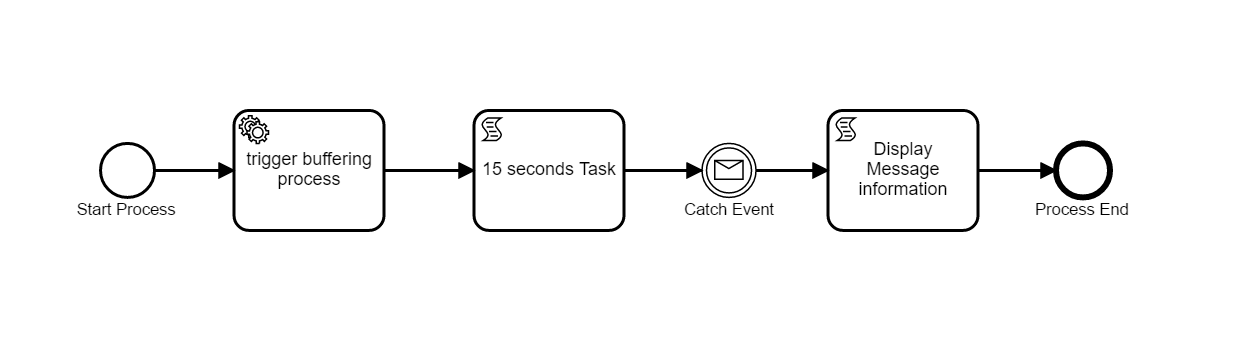
\includegraphics[width=1\linewidth]{chapters/assessment/example-o3.PNG}}
	\caption{Generic Example Process in Camunda for Occurrence Scenario \textit{O3}}\label{fig:camunda-example-o3}
\end{figure}

\begin{figure}[]
	\myfloatalign
	{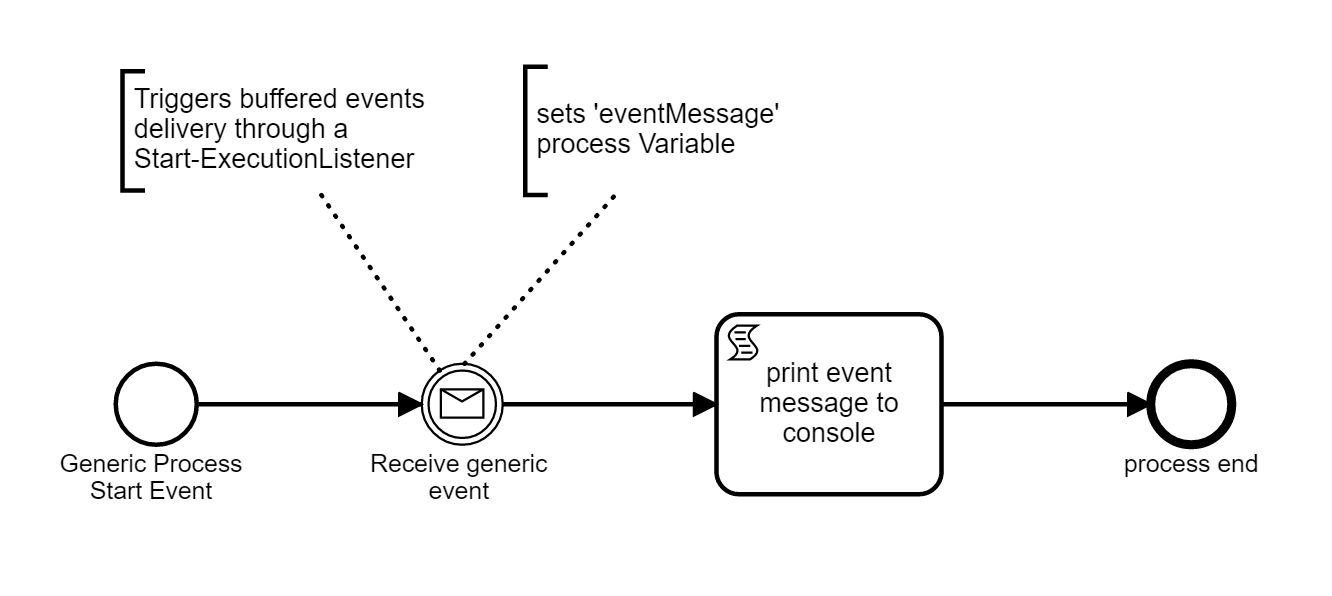
\includegraphics[width=1\linewidth]{chapters/assessment/example-o4-o5.PNG}}
	\caption{Generic Example Process in Camunda for Occurrence Scenarios \textit{O4} and \textit{O5}}\label{fig:camunda-example-o4-o5}
\end{figure}

\paragraph{Auxiliary Buffering Process}
The task of this process is to subscribe to a CEP Platform using a provided event query and start listening for events. Any incoming event must be stored in a data-store (\textit{Event Buffer}).
UNICORN, an Esper-based academic event processing platform, will be used in this example.
A local MySQL database has been chosen for buffering the event data because it's freely available, quick to set up, offers standardized access via SQL queries and Java connectors and will persist data to the local harddrive by default. As UNICORN also requires an SQL database, the MySQL instance can be used in both cases.

\autoref{fig:camunda-aux-buffering-process} shows the final Buffering Process modeled in the Camunda Process Modeler. The process can be instantiated by issuing a \textit{Buffering Task} message. This message must contain three data fields: \textit{processDefinitionId}, to know which process definition the buffered messages belong to; \textit{messageName}, the name of the message event within the process; \textit{query}, the event query in the Esper Query Language.
Camunda will make the message data automatically available in the process instance as process variables, so they can be used during the execution of the Buffering Process.
After instantiation, the process reaches the activity \textit{Subscribe to Event Source}, a \textit{Java Service Task} that executes a HTTP call to the UNICORN platform. That call registers the event query in UNICORN. \todo[inline]{it tells unicorn its own instanceId, so that unicorn can correlate events to that exact instance}
Afterwards, the process reaches the receiving activity \textit{Wait for unsubscribe event} that will terminate the process as soon as the \textit{Unsubscribe} event has been received.
As long as this activity is active, events can be received through the attached Non-Interrupting Boundary Event. Incoming events have a field \textit{eventBody}, which contains the event information and becomes available through a process variable with the same name. \todo[inline]{does the message from UC have a field 'eventBody'?}
The boundary event triggers the service task \textit{Write eventBody to datastore}, which takes the data from the process variable and writes it to the MySQL Database Instance (\textit{Global Event Buffer}).

\begin{figure}[]
	\myfloatalign
	{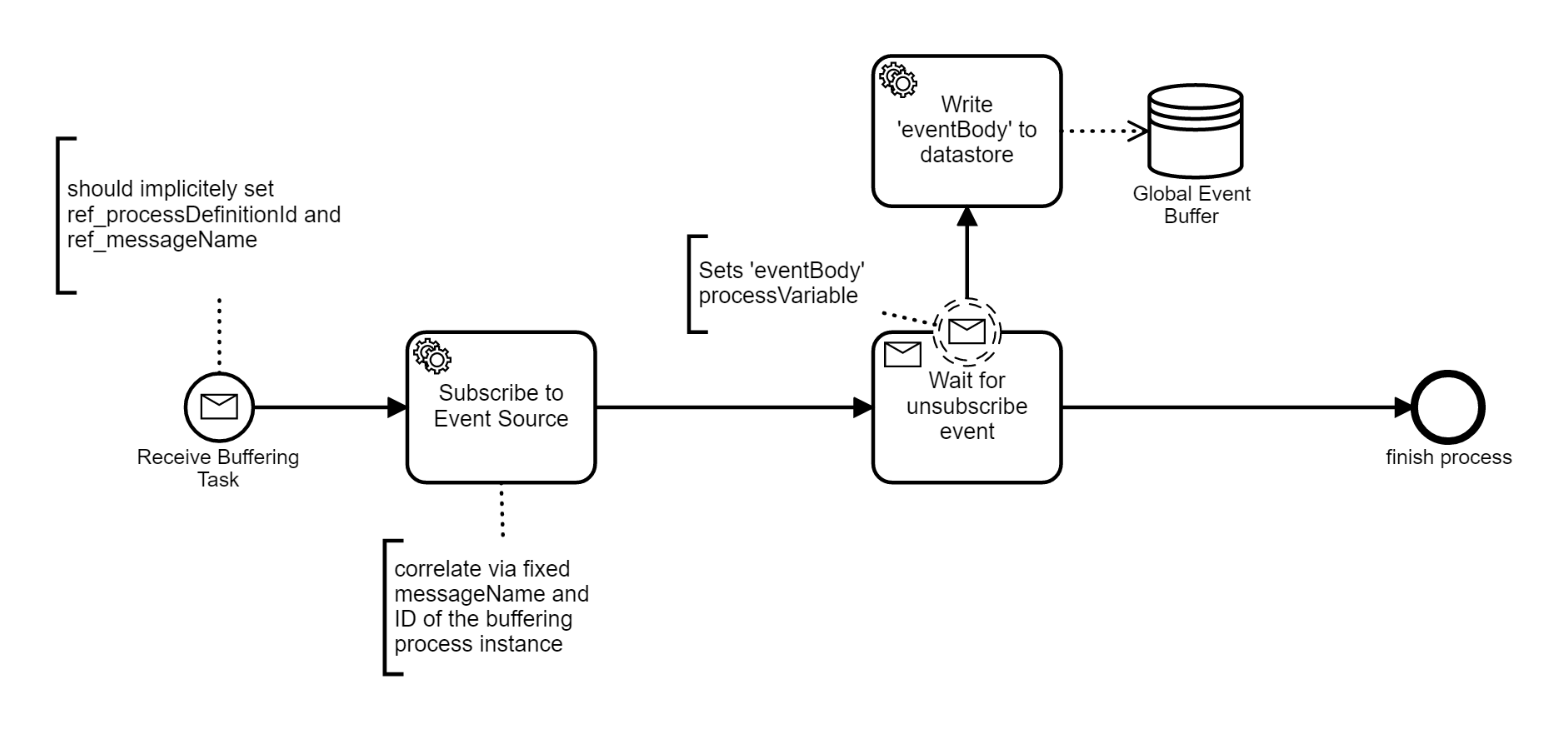
\includegraphics[width=1\linewidth]{chapters/assessment/buffering-process.PNG}}
	\caption{Auxiliary Buffering Process in the Camunda Modeler}\label{fig:camunda-aux-buffering-process}
\end{figure}

\paragraph{Auxiliary Event Delivery Process}
The delivery process (see \autoref{fig:camunda-aux-event-delivery}) reads the latest data from the buffer and sends it to the process instance. It can be started with a message that contains the \textit{processInstanceId} and the \textit{processDefinitionId} of the requesting process and the \textit{messageName} of the Message Event that is requested from the buffer.
A \textit{Delay} Timer Event has been inserted to make sure that the receiving process is already in listening state, the execution happens asynchronously.
It follows the service task \textit{Retrieve event from buffer}, which executes Java code to read from the MySQL Database \textit{Event Buffer} and store the event information in a process variable named \textit{eventMessage}.
The content of that process variable is sent to the \textit{Original Process} in the Send Event, afterwards the execution is finished.


\begin{figure}[]
	\myfloatalign
	{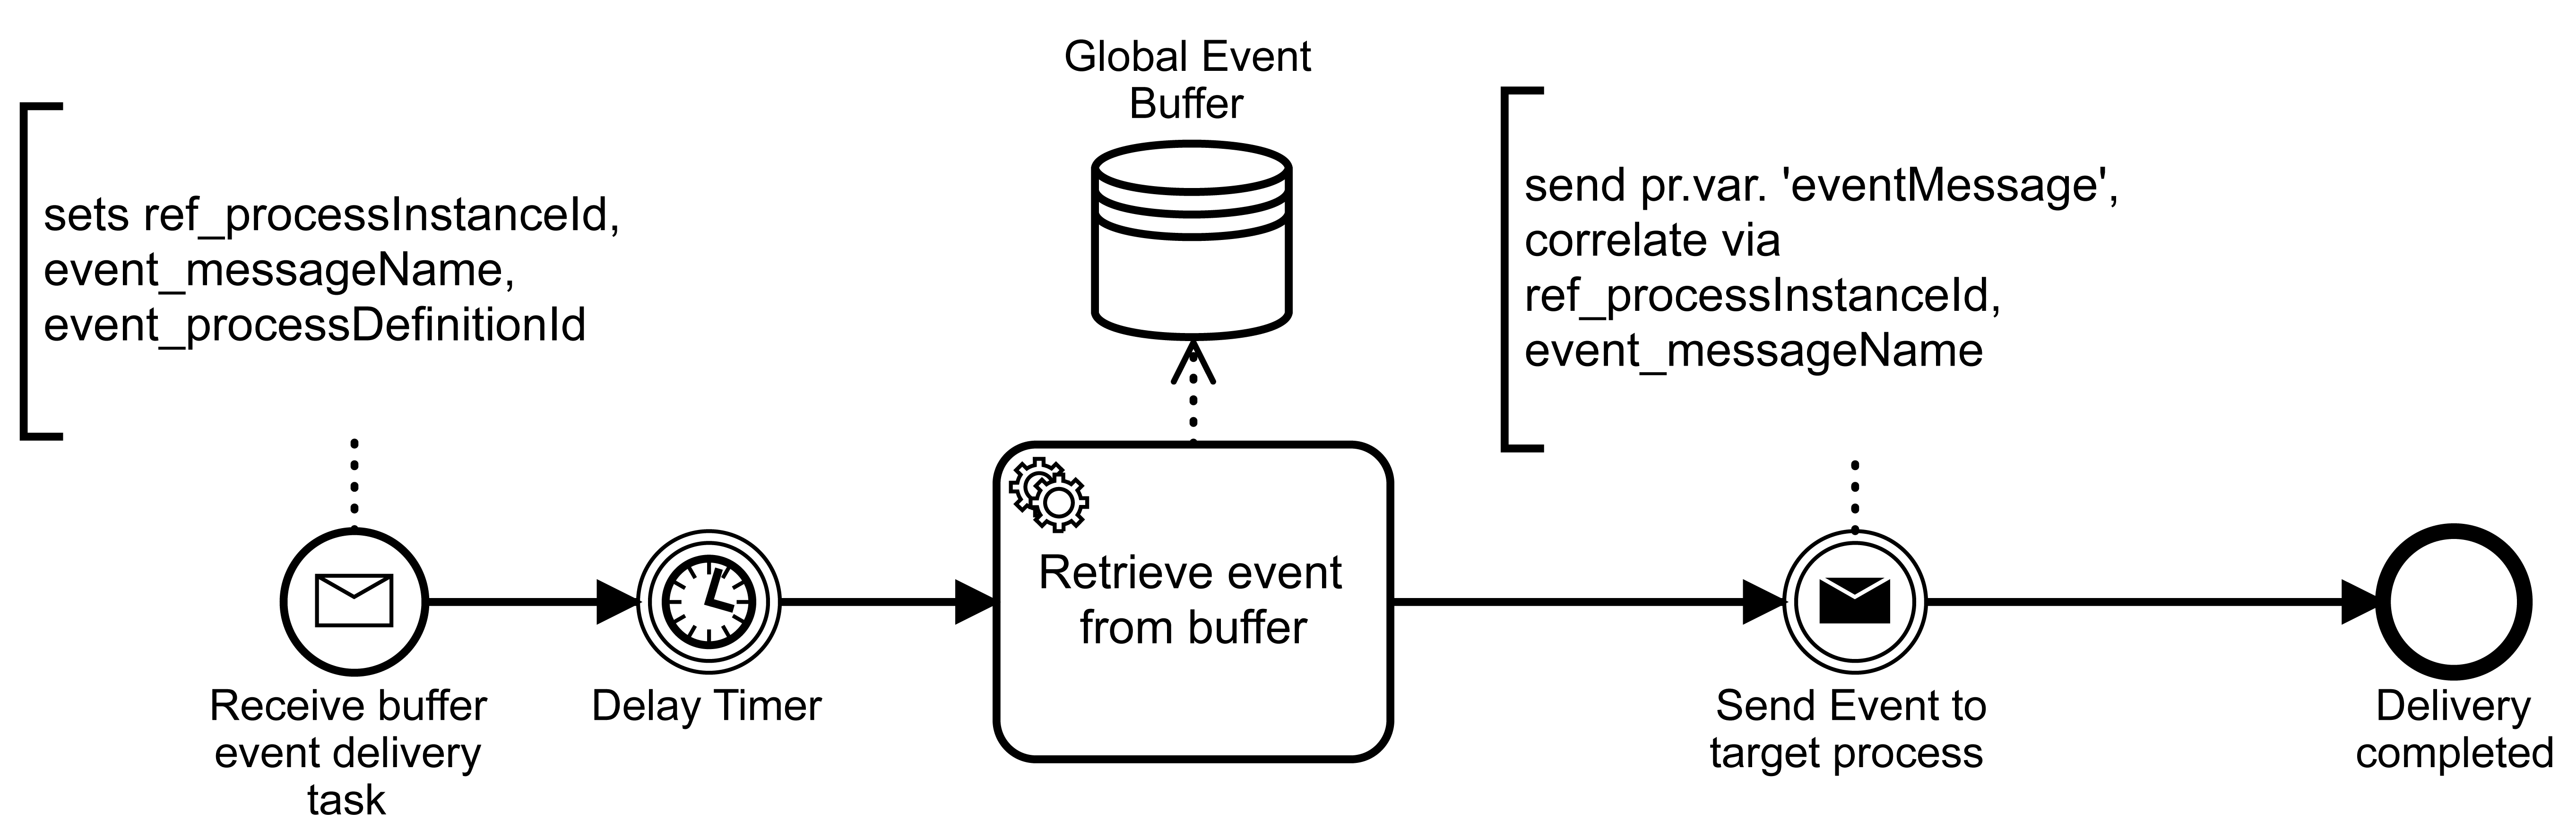
\includegraphics[width=1\linewidth]{chapters/assessment/buffer-delivery-process.PNG}}
	\caption{Auxiliary Event Delivery Process in Camunda Modeler}\label{fig:camunda-aux-event-delivery}
\end{figure}


\paragraph{Interaction of the Processes}
In this implementation of flexible event subscription, the action of subscribing to the event source and the reception of events in the Original Process are splitted into two separate parts, each supported by an auxiliary process.
To initiate the subscription at the event source, the Auxiliary Event Buffering process has to be started.
For scenario \textit{O3}, this happens through an extra activity (\textit{Trigger Buffering Process}) during process execution, so that events after process instantiation are received by the Buffering Process.
In scenarios \textit{O4} and \textit{O5}, the subscription and thus the instantiation of the Buffering Process must happen before the instantiation of the Target Process. As there is no such mechanism in the standard Camunda Process Engine, the Buffering Process must be started by hand, providing the \textit{processDefinitionId}, the \textit{messageName} and the \textit{eventQuery}.

Now that the \textit{Buffering Process} is running, any events matching the query will be stored to the buffer.
When the Target Process reaches the Catch Event, a request for buffered events is sent as a message to trigger the \textit{Auxiliary Event Delivery Process}.
This message is sent using a short piece of Java code that gets executed when the Catch Event is reached. 
The code is invoked by a Start ExecutionListener attached to the Catch Event. ExecutionListeners are offered by Camunda to execute own Java programs before or after relevant events during process execution, like the execution of an element in the process.
While the Original Process will now start listening for the desired events, the Event Delivery Process will send the buffered events as messages to the Original Process.

If no events have been received yet, all the involved processes remain active: the Buffering Process will keep listening for an external event. The Delivery Process will send an event to the Original Process as soon as there is one in the buffer. The Catch Event in the Original Process will keep listening for an Event.

\todo[inline]{the termination of the processes is not yet implemented in Camunda}
\todo[inline]{get wording straight: Original process, target process, requesting process, main process | also always italic or never}

\missingfigure{overview of the 3 processes, mysql and UNICORN}

\todo[inline]{note that this is an investigative implementation that matches exactly the given use-case and is not meant to be used in production. It is neither flexible nor robust enough for that purpose, but suits very well in understanding the capabilities and the shortcomings of BPMN and Camunda when it comes to handling the Event Occurrence Scenarios}


\section{Discussion}
The goal of this chapter was to get a better understanding of the capabilities of the tools when it comes to covering all event occurrence scenarios. 
Even though is has proven possible to to implement a flexible event subscription time using standard BPMN 2.0 and Camunda, the success comes at a cost.
The downsides of the presented approach are presented in the following.

It was necessary to create two generic auxiliary processes for event buffering, to connect to a MySQL data-store and use ExecutionListeners to execute custom Java code in Camunda to cover all scenarios, \textit{O1} to \textit{O5}.

\todo[inline]{give them short names for reference? Or make one of them Requirement 5}


\paragraph{Missing automatic subscription handling\newline}

In the presented process models, separate process elements had to be added to handle event subscription and initiate event delivery. 
That conflicts with requirement \textit{R2}, which states that the subscription and un-subscription must be automatically handled by the process engine.
For the scenarios \textit{O4} and \textit{O5} the Buffering Process has to be triggered manually, because it must be executed before the target process is running. Camunda does not handle external event subscription itself, especially not before the process is running.

\paragraph{Additional model complexity\newline}

As additional process elements have to be added to handle event subscription and delivery, the models become more complicated and are less concentrated on the business case.
\todo[inline]{there could be a requirement that states that there should be no additional process elements unless there is an explicit subscription time}

\paragraph{Buffering is an IT Task\newline}

The auxiliary processes are not business tasks and are thus not suited to be modeled in BPMN.
Desired functionality can be put into Camunda BPMN models thanks to its flexibility to use Java code in Service Tasks or Event Listeners, but naturally the full functionality of the Event Buffer cannot be expressed using BPMN.
\todo[inline]{what exactly is the issue here?}

\paragraph{Added load on the Process Engine\newline}

Because of the aux processes, two additional processes have to be deployed in the process engine and are potentially running in parallel to any given process instance. For each Event Element used in a process the engine has to run an instance of the Buffering Process and, eventually, an instance of the Buffer Delivery Process.
That puts additional load on the process engine, which might prevent business critical processes from executing delay-free.

Even when the number of deployed and running auxiliary processes can be reduced through further optimizations there remains an event-management overhead as every event has to be handled twice: once when it is stored in the buffer and once when it's delivered to the target process.

\paragraph{Hidden Performance Limitations of the Process Engine\newline}

Given the large amount and high frequency in that events can occur in reality, optimal performance is required for an event-buffering module.
Running essential parts of the buffering within the process engine might pose performance limitations that cannot be influenced without tempering with the process engine code.

\medskip \noindent
\todo[inline]{write connector to next chapter: it has been shown that... therefor we do ...}

